\documentclass[
  man,
  longtable,
  colorlinks=true,linkcolor=blue,citecolor=blue,urlcolor=blue]{apa7}


\ifLuaTeX
\usepackage[bidi=basic]{babel}
\else
\usepackage[bidi=default]{babel}
\fi
\babelprovide[main,import]{english}


% get rid of language-specific shorthands (see #6817):
\let\LanguageShortHands\languageshorthands
\def\languageshorthands#1{}

\RequirePackage{longtable}
% \setlength\LTleft{0pt}
\RequirePackage{threeparttablex}

% % % \RequirePackage{rotating}
% \RequirePackage{threeparttablex}
% \DeclareDelayedFloatFlavor{sidewaysfigure}{figure}
% \DeclareDelayedFloatFlavor{sidewaystable}{table}
% \DeclareDelayedFloatFlavor{longtable}{table}
\DeclareDelayedFloatFlavor{ThreePartTable}{table}


% % 


\makeatletter
\renewcommand{\paragraph}{\@startsection{paragraph}{4}{\parindent}%
	{0\baselineskip \@plus 0.2ex \@minus 0.2ex}%
	{-.5em}%
	{\normalfont\normalsize\bfseries\typesectitle}}

\renewcommand{\subparagraph}[1]{\@startsection{subparagraph}{5}{0.5em}%
	{0\baselineskip \@plus 0.2ex \@minus 0.2ex}%
	{-\z@\relax}%
	{\normalfont\normalsize\bfseries\itshape\hspace{\parindent}{#1}\textit{\addperi}}{\relax}}
\makeatother

\usepackage{amsmath}


\usepackage{longtable, booktabs, multirow, multicol, colortbl, hhline, caption, array, float}
\setcounter{topnumber}{2}
\setcounter{bottomnumber}{2}
\setcounter{totalnumber}{4}
\renewcommand{\topfraction}{0.85}
\renewcommand{\bottomfraction}{0.85}
\renewcommand{\textfraction}{0.15}
\renewcommand{\floatpagefraction}{0.7}

\usepackage{tcolorbox}
\tcbuselibrary{listings,theorems, breakable, skins}
\usepackage{fontawesome5}

\definecolor{quarto-callout-color}{HTML}{909090}
\definecolor{quarto-callout-note-color}{HTML}{0758E5}
\definecolor{quarto-callout-important-color}{HTML}{CC1914}
\definecolor{quarto-callout-warning-color}{HTML}{EB9113}
\definecolor{quarto-callout-tip-color}{HTML}{00A047}
\definecolor{quarto-callout-caution-color}{HTML}{FC5300}
\definecolor{quarto-callout-color-frame}{HTML}{ACACAC}
\definecolor{quarto-callout-note-color-frame}{HTML}{4582EC}
\definecolor{quarto-callout-important-color-frame}{HTML}{D9534F}
\definecolor{quarto-callout-warning-color-frame}{HTML}{F0AD4E}
\definecolor{quarto-callout-tip-color-frame}{HTML}{02B875}
\definecolor{quarto-callout-caution-color-frame}{HTML}{FD7E14}


% 

\newlength\Oldarrayrulewidth
\newlength\Oldtabcolsep


\usepackage{hyperref}




\providecommand{\tightlist}{%
  \setlength{\itemsep}{0pt}\setlength{\parskip}{0pt}}
\usepackage{longtable,booktabs,array}
\usepackage{calc} % for calculating minipage widths
% Correct order of tables after \paragraph or \subparagraph
\usepackage{etoolbox}
\makeatletter
\patchcmd\longtable{\par}{\if@noskipsec\mbox{}\fi\par}{}{}
\makeatother
% Allow footnotes in longtable head/foot
\IfFileExists{footnotehyper.sty}{\usepackage{footnotehyper}}{\usepackage{footnote}}
\makesavenoteenv{longtable}

\usepackage{graphicx}
\makeatletter
\def\maxwidth{\ifdim\Gin@nat@width>\linewidth\linewidth\else\Gin@nat@width\fi}
\def\maxheight{\ifdim\Gin@nat@height>\textheight\textheight\else\Gin@nat@height\fi}
\makeatother
% Scale images if necessary, so that they will not overflow the page
% margins by default, and it is still possible to overwrite the defaults
% using explicit options in \includegraphics[width, height, ...]{}
\setkeys{Gin}{width=\maxwidth,height=\maxheight,keepaspectratio}
% Set default figure placement to htbp
\makeatletter
\def\fps@figure{htbp}
\makeatother


% definitions for citeproc citations
\NewDocumentCommand\citeproctext{}{}
\NewDocumentCommand\citeproc{mm}{%
  \begingroup\def\citeproctext{#2}\cite{#1}\endgroup}
\makeatletter
 % allow citations to break across lines
 \let\@cite@ofmt\@firstofone
 % avoid brackets around text for \cite:
 \def\@biblabel#1{}
 \def\@cite#1#2{{#1\if@tempswa , #2\fi}}
\makeatother
\newlength{\cslhangindent}
\setlength{\cslhangindent}{1.5em}
\newlength{\csllabelwidth}
\setlength{\csllabelwidth}{3em}
\newenvironment{CSLReferences}[2] % #1 hanging-indent, #2 entry-spacing
 {\begin{list}{}{%
  \setlength{\itemindent}{0pt}
  \setlength{\leftmargin}{0pt}
  \setlength{\parsep}{0pt}
  % turn on hanging indent if param 1 is 1
  \ifodd #1
   \setlength{\leftmargin}{\cslhangindent}
   \setlength{\itemindent}{-1\cslhangindent}
  \fi
  % set entry spacing
  \setlength{\itemsep}{#2\baselineskip}}}
 {\end{list}}
\usepackage{calc}
\newcommand{\CSLBlock}[1]{\hfill\break\parbox[t]{\linewidth}{\strut\ignorespaces#1\strut}}
\newcommand{\CSLLeftMargin}[1]{\parbox[t]{\csllabelwidth}{\strut#1\strut}}
\newcommand{\CSLRightInline}[1]{\parbox[t]{\linewidth - \csllabelwidth}{\strut#1\strut}}
\newcommand{\CSLIndent}[1]{\hspace{\cslhangindent}#1}


\usepackage{times}
    


\title{Using Quarto to Generate Documents in APA Style (7th Edition)}
\shorttitle{Template for the apaquarto Extension}


\usepackage{etoolbox}






\authorsnames[{1},{1},{2,3},{4}]{
Ana Fulano,Blanca Zutano,Carina Mengano,Dolorita Perengano
}



\authorsaffiliations{
{Department of Psychology, Ana and Blanca's University},{Carina's
Primary Affiliation},{Carina's Secondary Affiliation},{Buffalo, NY }}






\leftheader{Fulano, Zutano, Mengano and Perengano}



\abstract{This document is a template demonstrating the apaquarto
format.}
% 
\keywords{keyword1, keyword2, keyword3}

\authornote{\par{\addORCIDlink{Ana
Fulano}{0000-0000-0000-0001}}\par{\addORCIDlink{Blanca
Zutano}{0000-0000-0000-0002}}\par{\addORCIDlink{Carina
Mengano}{0000-0000-0000-0003}}\par{\addORCIDlink{Dolorita
Perengano}{0000-0000-0000-0004}}
\par{ }
\par{       Author roles were classified using the Contributor Role Taxonomy (CRediT; https://credit.niso.org/) as follows: Ana
Fulano:   conceptualization, writing; Blanca Zutano:   project
administration, formal analysis; Carina Mengano:   formal
analysis, writing; Dolorita Perengano:   writing, methodology, formal
analysis}
\par{Correspondence concerning this article should be addressed to Ana
Fulano, Department of Psychology, Ana and Blanca's University, 1234
Capital St., Albany, NY 12084-1234, Email: sm@example.org}
}


\makeatletter
\let\endoldlt\endlongtable
\def\endlongtable{
\hline
\endoldlt
}
\makeatother
\RequirePackage{longtable}
\DeclareDelayedFloatFlavor{longtable}{table}
% \RequirePackage{threeparttablex}
% \DeclareDelayedFloatFlavor{ThreePartTable}{table}

\urlstyle{same}





\begin{document}
\maketitle
\setcounter{secnumdepth}{-\maxdimen} % remove section numbering

\setlength\LTleft{0pt}


This is my introductory paragraph. The title will be placed above it
automatically. \emph{Do not start with an introductory heading} (e.g.,
``Introduction''). The title acts as your Level 1 heading for the
introduction.

Details about writing headings with markdown in APA style are
\href{https://wjschne.github.io/apaquarto/writing.html\#headings-in-apa-style}{here}.

\subsection{Displaying Figures}\label{displaying-figures}

A reference label for a figure must have the prefix \texttt{fig-}, and
in a code chunk, the caption must be set with \texttt{fig-cap}. Captions
are in
\href{https://apastyle.apa.org/style-grammar-guidelines/capitalization/title-case}{title
case}.

\begin{figure}[!htbp]

{\caption{{The Figure Caption}{\label{fig-myplot}}}}

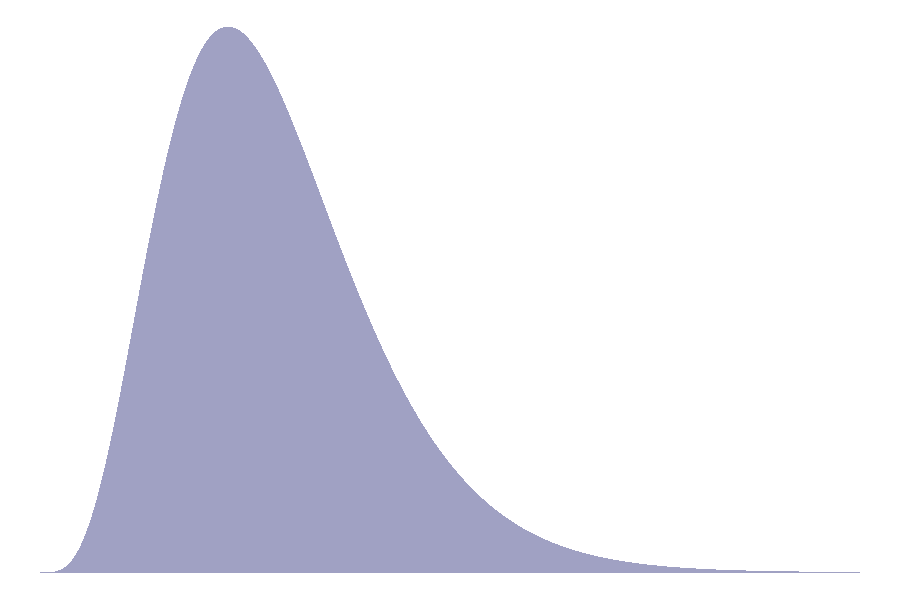
\includegraphics{template_files/figure-pdf/fig-myplot-1.pdf}

{\noindent \emph{Note.} This is the note below the figure.}

\end{figure}

To refer to any figure or table, use the \texttt{@} symbol followed by
the reference label (e.g., Figure~\ref{fig-myplot}).

\subsection{Imported Graphics}\label{imported-graphics}

One way to import an existing graphic as a figure is to use
\texttt{knitr::include\_graphics} in a code chunk. For example,
Figure~\ref{fig-import1} is an imported image. Note that in
apaquarto-pdf documents, we can specify that that a figure or table
should span both columns when in journal mode by setting the
\texttt{apa-twocolumn} chunk option to \texttt{true}. For other formats,
this distinction does not matter.

\begin{figure*}[!htbp]

{\caption{{An Imported Graphic}{\label{fig-import1}}}}

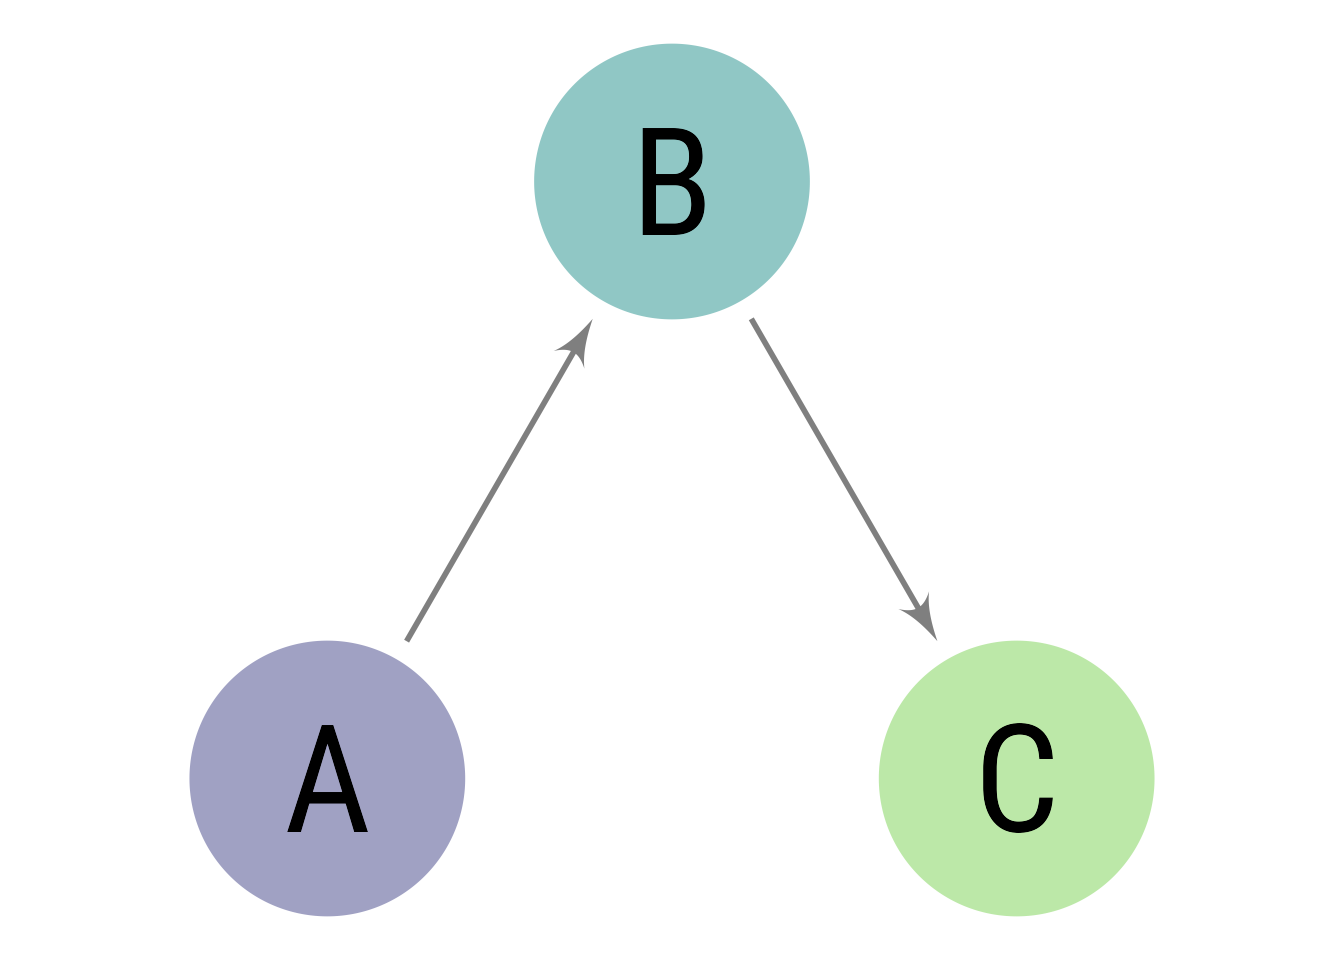
\includegraphics[width=1\textwidth,height=\textheight]{img/sampleimage.png}

{\noindent \emph{Note.} A note below the figure}

\end{figure*}

Figure graphics can be imported directly with Markdown:

\begin{figure}[!htbp]

{\caption{{Another Way to Import Graphics}{\label{fig-import2}}}}

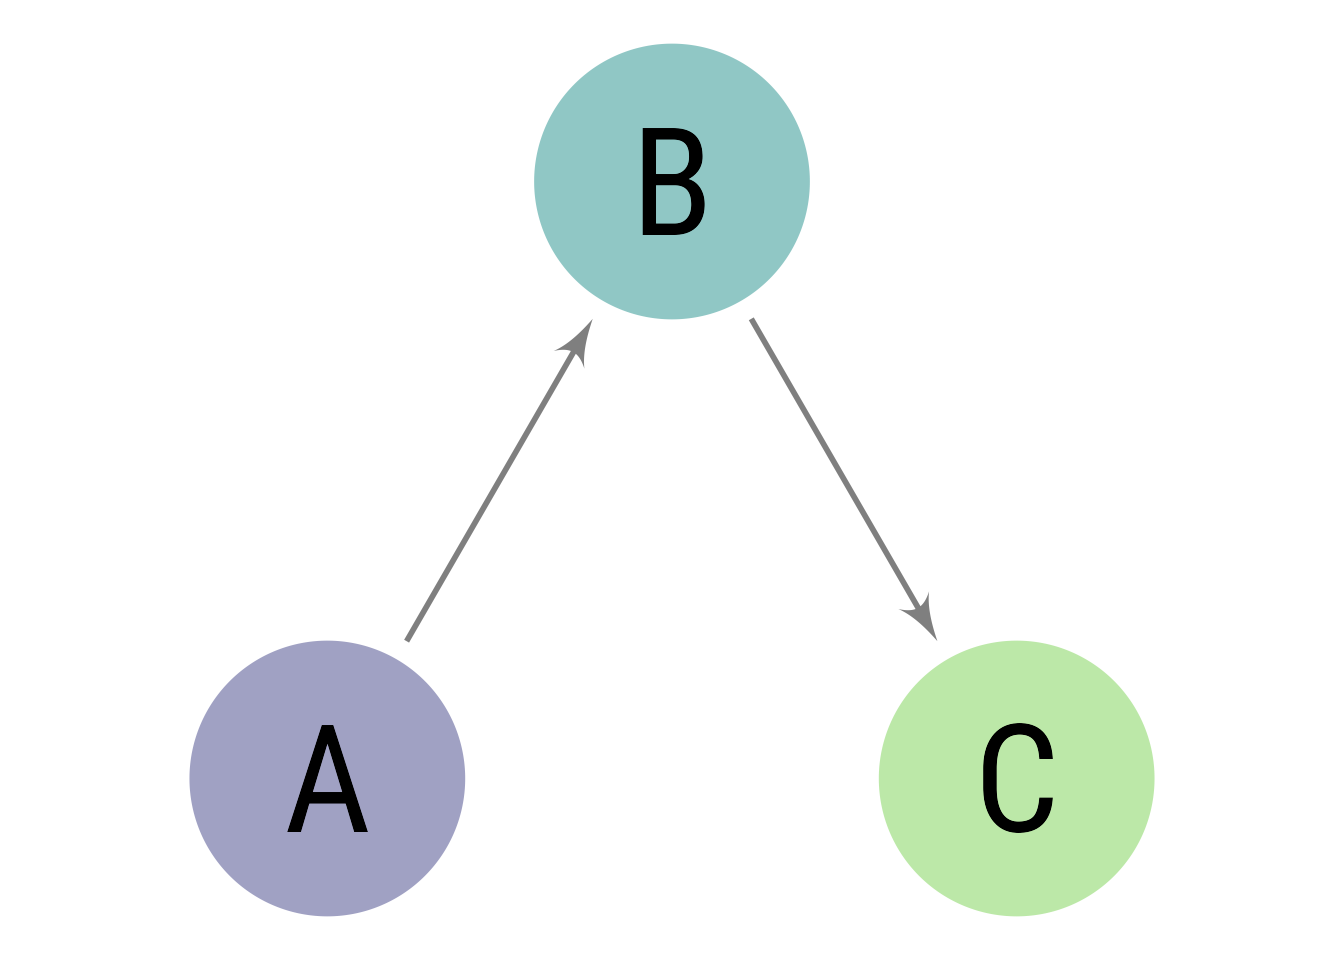
\includegraphics{img/sampleimage.png}

{\noindent \emph{Note.} A note below the figure}

\end{figure}

\subsection{Displaying Tables}\label{displaying-tables}

We can make a table the same way as a figure. Generating a table that
conforms to APA format in all document formats can be tricky. When the
table is simple, the \texttt{kable} function from knitr works well. Feel
free to experiment with different methods, but I have found that David
Gohel's \href{https://davidgohel.github.io/flextable/}{flextable} to be
the best option when I need something more complex.

\begin{table}

{\caption{{The Table Caption}{\label{tbl-mytable}}}
\vspace{-20pt}}

\global\setlength{\Oldarrayrulewidth}{\arrayrulewidth}

\global\setlength{\Oldtabcolsep}{\tabcolsep}

\setlength{\tabcolsep}{2pt}

\renewcommand*{\arraystretch}{1.5}



\providecommand{\ascline}[3]{\noalign{\global\arrayrulewidth #1}\arrayrulecolor[HTML]{#2}\cline{#3}}

\begin{longtable*}[l]{|p{0.75in}|p{0.75in}}



\ascline{0.75pt}{000000}{1-2}

\multicolumn{1}{>{\centering}m{\dimexpr 0.75in+0\tabcolsep}}{\textcolor[HTML]{000000}{\fontsize{11}{11}\selectfont{Numbers}}} & \multicolumn{1}{>{\centering}m{\dimexpr 0.75in+0\tabcolsep}}{\textcolor[HTML]{000000}{\fontsize{11}{11}\selectfont{Letters}}} \\

\ascline{0.75pt}{000000}{1-2}\endfirsthead 

\ascline{0.75pt}{000000}{1-2}

\multicolumn{1}{>{\centering}m{\dimexpr 0.75in+0\tabcolsep}}{\textcolor[HTML]{000000}{\fontsize{11}{11}\selectfont{Numbers}}} & \multicolumn{1}{>{\centering}m{\dimexpr 0.75in+0\tabcolsep}}{\textcolor[HTML]{000000}{\fontsize{11}{11}\selectfont{Letters}}} \\

\ascline{0.75pt}{000000}{1-2}\endhead



\multicolumn{1}{>{\centering}m{\dimexpr 0.75in+0\tabcolsep}}{\textcolor[HTML]{000000}{\fontsize{11}{11}\selectfont{1}}} & \multicolumn{1}{>{\centering}m{\dimexpr 0.75in+0\tabcolsep}}{\textcolor[HTML]{000000}{\fontsize{11}{11}\selectfont{A}}} \\





\multicolumn{1}{>{\centering}m{\dimexpr 0.75in+0\tabcolsep}}{\textcolor[HTML]{000000}{\fontsize{11}{11}\selectfont{2}}} & \multicolumn{1}{>{\centering}m{\dimexpr 0.75in+0\tabcolsep}}{\textcolor[HTML]{000000}{\fontsize{11}{11}\selectfont{B}}} \\





\multicolumn{1}{>{\centering}m{\dimexpr 0.75in+0\tabcolsep}}{\textcolor[HTML]{000000}{\fontsize{11}{11}\selectfont{3}}} & \multicolumn{1}{>{\centering}m{\dimexpr 0.75in+0\tabcolsep}}{\textcolor[HTML]{000000}{\fontsize{11}{11}\selectfont{C}}} \\





\multicolumn{1}{>{\centering}m{\dimexpr 0.75in+0\tabcolsep}}{\textcolor[HTML]{000000}{\fontsize{11}{11}\selectfont{4}}} & \multicolumn{1}{>{\centering}m{\dimexpr 0.75in+0\tabcolsep}}{\textcolor[HTML]{000000}{\fontsize{11}{11}\selectfont{D}}} \\

\ascline{0.75pt}{000000}{1-2}



\end{longtable*}



\arrayrulecolor[HTML]{000000}

\global\setlength{\arrayrulewidth}{\Oldarrayrulewidth}

\global\setlength{\tabcolsep}{\Oldtabcolsep}

\renewcommand*{\arraystretch}{1}

{\vspace{-20pt}
\noindent \emph{Note.} The note below the table.}

\end{table}

To refer to this table in text, use the \texttt{@} symbol followed by
the reference label like so: As seen in Table~\ref{tbl-mytable}, the
first few numbers and letters of the alphabet are displayed.

In Table~\ref{tbl-mymarkdowntable}, there is an example of a plain
markdown table with a note below it.

\begin{table}

{\caption{{Table Caption of a Markdown
Table}{\label{tbl-mymarkdowntable}}}
\vspace{-20pt}}

\begin{longtable}[]{@{}llrc@{}}
\toprule\noalign{}
Default & Left & Right & Center \\
\midrule\noalign{}
\endhead
\bottomrule\noalign{}
\endlastfoot
12 & 12 & 12 & 12 \\
123 & 123 & 123 & 123 \\
1 & 1 & 1 & 1 \\
\end{longtable}

{\vspace{-20pt}
\noindent \emph{Note.} This is a note below the markdown table.}

\end{table}

What if you want the tables and figures to be at the end of the
document? In the .pdf format, you can set the \texttt{floatsintext}
option to false. For .html and .docx documents, there is not yet an
automatic way to put tables and figures at the end. You can, of course,
just put them all at the end, in order. The reference labels will work
no matter where they are in the text.

\subsection{Citations}\label{citations}

See
\href{https://quarto.org/docs/authoring/footnotes-and-citations.html}{here}
for instructions on setting up citations and references.

A parenthetical citation requires square brackets (Cameron \& Trivedi,
2013). This reference was in my bibliography file. An in-text citation
is done like so: Cameron and Trivedi (2013).

See
\href{https://wjschne.github.io/apaquarto/writing.html\#references}{here}
for explanations, examples, and citation features exclusive to apaquarto
like masked citations (citations masked for peer review) and possessive
citations (e.g., ``Schneider and McGrew's (2012) idea seemed reasonable
at the time.'')

\subsection{Masking Author Identity for Peer
Review}\label{masking-author-identity-for-peer-review}

Setting \texttt{mask} to \texttt{true} will remove author names,
affiliations, and correspondence from the title page. Any references
listed in the \texttt{masked-citations} field will be masked as well.
See
\href{https://wjschne.github.io/apaquarto/writing.html\#masked-citations-for-anonymous-peer-review}{here}
for more information.

\subsection{Hypotheses, Aims, and
Objectives}\label{hypotheses-aims-and-objectives}

The last paragraph of the introduction usually states the specific
hypotheses of the study, often in a way that links them to the research
design.

\section{Method}\label{method}

General remarks on method. This paragraph is optional.

Not all papers require each of these sections. Edit them as needed.
Consult the \href{https://apastyle.apa.org/jars}{Journal Article
Reporting Standards} for what is needed for your type of article.

\subsection{Participants}\label{participants}

Who are they? How were they recruited? Report criteria for participant
inclusion and exclusion. Perhaps some basic demographic stats are in
order. A table is a great way to avoid repetition in statistical
reporting.

\subsection{Measures}\label{measures}

This section can also be titled \textbf{Materials} or
\textbf{Apparatus}. Whatever tools, equipment, or measurement devices
used in the study should be described.

\subsubsection{Measure A}\label{measure-a}

Describe Measure A.

\subsubsection{Measure B}\label{measure-b}

Describe Measure B.

\subsection{Procedure}\label{procedure}

What did participants do?

How are the data going to be analyzed?

\section{Results}\label{results}

\subsection{Descriptive Statistics}\label{descriptive-statistics}

Here we describe the basic characteristics of our primary variables.

\section{Discussion}\label{discussion}

Describe results in non-statistical terms.

\subsection{Limitations and Future
Directions}\label{limitations-and-future-directions}

Every study has limitations. Based on this study, some additional steps
might include\ldots{}

\subsection{Conclusion}\label{conclusion}

Let's sum this up.

\section{References}\label{references}

\phantomsection\label{refs}
\begin{CSLReferences}{1}{0}
\bibitem[\citeproctext]{ref-CameronTrivedi2013}
Cameron, A. C., \& Trivedi, P. K. (2013). \emph{Regression analysis of
count data} (2nd ed.). Cambridge University Press.
\url{https://doi.org/10.1017/CBO9781139013567}

\bibitem[\citeproctext]{ref-schneider2012cattell}
Schneider, W. J., \& McGrew, K. S. (2012). \emph{The
{Cattell-Horn-Carroll} model of intelligence.}

\end{CSLReferences}

\section{Appendix}\label{appendix}

If there are multiple appendices, label them with level 1 headings as
Appendix A, Appendix B, and so forth.





\end{document}
